% -----------------------------------------------------
% QUESTION
% -----------------------------------------------------
\question 
Write the main text for the question here. This is an example of an inline equation: $F=ma$, where $F$ is the force, or $E=\frac{1}{2}mv^2$. For SI units use: the force is $F=1.0$~\si{N} or $F=\SI{2.0}{\newton}$ and the velocity is $v=\SI{3.4}{\meter\per\second}$. To add a table to the questions use:
%
\begin{table}[h!]
    \centering
    \label{tab:my_label}
    \caption{This is the caption for this table.}
\begin{tabular}{lrr}  
\toprule
\multicolumn{2}{c}{Item} \\
\cmidrule(r){1-2}
Property        & Value         & Units         \\ \midrule
Force           & \num{1.0}     & \si{N}        \\
Acceleration    & \num{3.4}     & \si{m/s^2}    \\
Temperature     & \num{-250}    & \si{K}        \\
Energy          & \num{200}     & \si{J}    \\
Potatoes        & Frozen        & Count         \\
\bottomrule
\end{tabular}
\addtocounter{table}{-1}
\end{table}

With this version of the exam paper template it is also possible to add chemical symbols such as \ce{H2O} or displayed chemical symbols or reactions, such as
 %
 \[ \ce{x Na(NH4)HPO4 ->[\Delta] (NaPO3)_x + x NH3 ^ + x H2O} \]

\begin{parts}	
% -----------------------------------------------------
\part This is the text of a part of a question ... % EDIT - Number of points between brackets

\begin{subparts}
\subpart[7] This is a subpart of a question
\droppoints

\subpart[3] And this is another subpart of a question, another subpart of a question. And this is another subpart of a question. And this is another subpart of a question. And this is another subpart of a question. 
\droppoints

\end{subparts}

\begin{solution}
This is an example solution ... and you can include a handwritten solution if you prefer.

% -----------------------------------------------------
% To include a handwritten solution, scan or photograph
% it and save it in the Images folder. Then use the 
% following code to include it in the exam paper,
% simply change the name of the image file within the
% \includegraphics LaTeX command.
% -----------------------------------------------------
\begin{center}
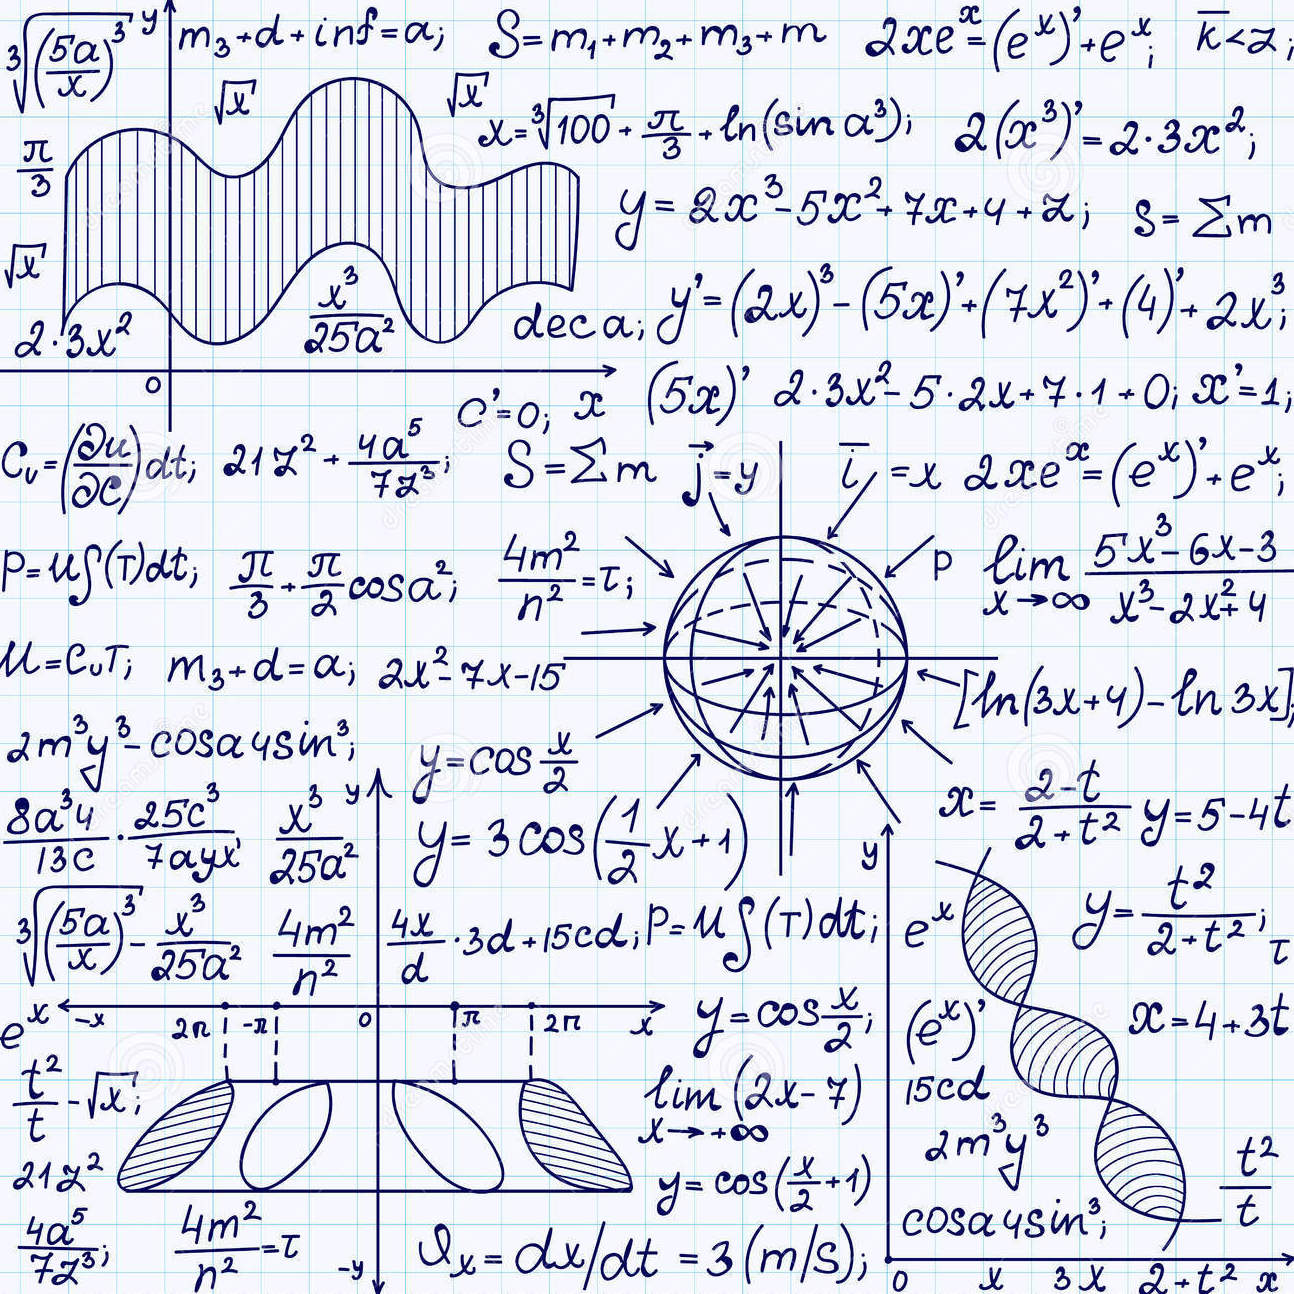
\includegraphics[width=0.95\textwidth]{Handwritten-solutions.jpg}
\end{center}


%
\end{solution}

% -----------------------------------------------------
\part[5] This is the text of a part of a question ... % EDIT - Number of points between brackets
\droppoints

\begin{solution}
This is an example solution ...
%
\end{solution}

% -----------------------------------------------------
\part[5] This is the text of a part of a question ... % EDIT - Number of points between brackets
\droppoints

\begin{solution}
This is an example solution ...
%
\end{solution}

\end{parts}

\begin{figure}[!ht]  
   \centering
   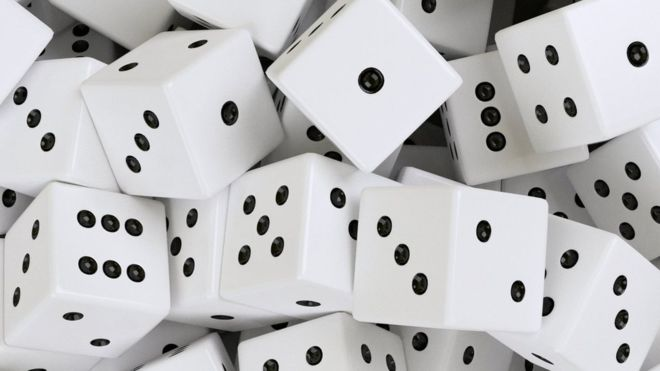
\includegraphics[width=0.8\textwidth]{RandomImage.jpg}
%   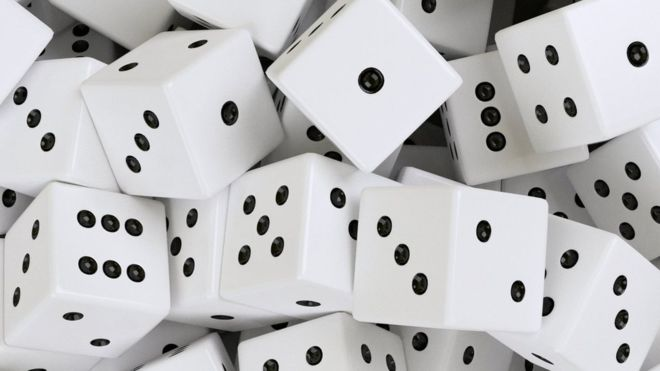
\includegraphics[height=60mm]{RandomImage.jpg}
   \caption{This is the caption for this question.}
   \label{fig:questionA1}                             % EDIT - Create unique labels for figures
    \addtocounter{figure}{-1}
\end{figure}
